
\section{Introduction}
%solar wind beginnings
From observations of cometary tail fluctuations \citet{Biermann1951} inferred the presence of a continuous flow of particles from the Sun. With his theoretical solar wind model \citet{Parker1958} formulated the existence of the solar wind even before the first satellites measured it in situ in 1959 \citep{Gringauz1960,Neugebauer1966}.
%in situ spacecraft
The idea of a space mission flying through the solar corona dates back to the founding year of NASA in 1958 \citep{McComas2008}. Since then several space missions have measured the solar wind in situ at a wide range of heliocentric distances, in case of Voyager~1 as far away as \SI{138}{\au}\footnote{\url{https://voyager.jpl.nasa.gov/}} (July 2017), having even left the heliospause into interstellar space at a distance of \SI{121}{\au} \citep{Gurnett2013}.
Until today various spacecraft have provided a wealth of solar wind measurements near Earth’s orbit, with WIND \citep{Lepping1995,Ogilvie1995}, ACE \citep{Stone1998} and DSCOVR \citep{Burt2012} still orbiting around the L1 point \SI{1.5}{million\,\km} ahead of Earth in the sunward direction. Additional measurements at other solar distances were provided by planetary missions to Venus and Mercury, such as PVO \citep{Colin1980} or MESSENGER \citep{Belcher1991}. Ulysses was the first probe that orbited the Sun out of the ecliptic plane and thus could measure solar wind even at polar latitudes \citep{McComas1998}. The Sun-nearest in situ solar wind measurements to date were obtained by the Helios mission. The in 1974 launched Helios~1 spacecraft reached distances of \SI{0.31}{\au}, Helios~2 launched two years later and approached the Sun up to \SI{0.29}{\au} \citep{Rosenbauer1977}.
%Solar Probe Plus mission
The NASA Parker~Solar~Probe\footnote{\url{http://parkersolarprobe.jhuapl.edu/}} (PSP), formerly Solar~Probe~Plus, with a planned launch date in mid 2018, will reach after six years in 2024 its closest perihelia at a distance of 9.86~solar radii (\Rs), that is, \SI{0.0459}{\au} \citep{Fox2015}. This distance will be achieved through seven Venus gravity assists with orbital periods of 88--168~days. In its prime mission time 2018--2025 PSP provides 24~orbits with perihelia inside \SI{0.25}{\au} \citep{Fox2015}. Even its first perihelion, 93~days after launch in 2018, will take PSP to an unprecedented distance of \SI{0.16}{\au} (\SI{35.7}{\Rs}). In comparison, the ESA Solar Orbiter mission with a planned launch in February 2019 will have its closest perihelia at \SI{0.28}{\au} \citep{Muller2013}.

%PSP objectives and instruments
The key PSP science objectives are to “trace the flow of energy that heats and accelerates the solar corona and solar wind, determine the structure and dynamics of the plasma and magnetic fields at the sources of the solar wind, and explore mechanisms that accelerate and transport energetic particles” as stated in \citet{Fox2015}. To achieve these goals, PSP has four scientific instruments on board: FIELDS for the measurements of magnetic fields and AC/DC electric fields \citep{Bale2016}, SWEAP for the measurements of flux of electrons, protons and alphas \citep{Kasper2016}, IS\sun{}IS for the measurement of solar energetic particles \citep{McComas2016} and WISPR for the measurement of coronal and inner heliospheric structures \citep{Vourlidas2016}.

%CGAUSS and WISPR
The study presented in this paper is undertaken in the Coronagraphic German And US Solar Probe Survey (CGAUSS) project, which is the German contribution to the PSP mission as part of the Wide field Imager for Solar PRobe (WISPR). WISPR will contribute to the PSP science goals by deriving the 3D structure of the solar corona through which the in situ measurements are made to determine the sources of the solar wind. It will provide density power spectra over a wide range of structures (e.g., streamers, pseudostreamers and equatorial coronal holes) for determining the roles of turbulence, waves and pressure-balanced structures in the solar wind. It will also measure the physical properties, such as speed and density jumps of SEP-producing shocks and their CME drivers as they evolve in the corona and inner heliosphere \citep{Vourlidas2016}.

In order to help optimize the WISPR and PSP preplanning of the science operations knowledge of the expected solar wind environment is needed. For this purpose the solar wind environment is extrapolated down to the closest perihelion of \SI{9.86}{\Rs} distance to the Sun using in situ solar wind data from the Helios probes and near \SI{1}{\au} data from various satellites compiled in the OMNI solar wind database.


%definition of sw environment
%section{Solar wind}
Generally, two types of solar wind are observed in the heliosphere, slow and fast streams \citep{Neugebauer1966,Schwenn1983}. Slow solar wind has typical speeds \SI{<400}{\km\per\s} and fast solar wind has speeds \SI{>600}{\km\per\s} \citep[p.~144]{Schwenn1990}. Their different compositions and characteristics indicate different sources and generation processes \citep{McGregor2011a}. Fast streams are found to originate from coronal holes as confirmed by Ulysses' out-of-ecliptic measurements \citep{McComas1998}. The source of slow wind and its eventually different types \citep{Schwenn1983}, is still a subject of controversial discussions because several scenarios are possible to explain its origin from closed magnetic structures in the solar corona, such as intermittent reconnection at the top of helmet streamers and from coronal hole boundaries \citep{Kilpua2016}. The occurrence frequency of these slow and fast streams varies strongly with solar activity and their interactions lead to phenomena such as stream interaction regions and for quasi-stationary coronal source regions to co-rotating interaction regions \citep{Balogh1999}.
Embedded in the slow and fast solar wind streams are transient flows of coronal mass ejections (CMEs), the faster ones driving shock waves ahead \citep{Gosling1974}. Their rate follows the solar activity cycle and varies in near \SI{1}{\au} measurements between only one CME every couple of days during solar cycle minima up to multiple CMEs observed over several days at times of solar maxima, that is, the CME-associated flow share of the solar wind raises from about \SI{5}{\percent} up to about \SI{50}{\percent} \citep{Richardson2012}.

%solar wind parameters
It is not known which specific solar wind type or structure PSP will encounter at a given time during its mission, therefore we extrapolate the probability distributions of the major solar wind parameters from existing solar wind measurements and take solar cycle dependencies into account.
As a baseline we describe the solar wind environment through the key quantities of a magnetized plasma: \textit{density}, \textit{temperature} and \textit{magnetic field strength}. Furthermore, the bulk flow \textit{velocity} is the defining parameter of the two types of solar wind. Solar wind quantities, like flux densities, mass flux and plasma beta, can directly be derived from these four parameters.

%sections
Our approach is to obtain analytical representations of the shapes of the solar wind parameter’s frequency distributions in Sect.~\ref{sec:frequency_distribution}, of their solar activity dependence in Sect.~\ref{sec:solar_activity_variations} and of their solar distance scaling in Sect.~\ref{sec:solar_distance_dependency}. The solar wind parameters’ frequency distributions and solar activity dependence is derived from near-Earth solar wind and sunspot number (SSN) time series with a duration of almost five solar cycles. Their distance dependency is derived from Helios solar wind measurements covering more than two third of the distance to the Sun and more than half a solar cycle. From combination of the obtained frequency distributions, SSN dependence functions and solar distance dependence functions a general solar wind model is build in Sect.~\ref{sec:empirical_solar_wind_model}, representing the solar activity and distance behavior. Finally, this empirical model is fed with a SSN prediction and extrapolated to PSP's planned orbital positions in Sect.~\ref{sec:model_extrapolation_to_psp_orbit}.


%lognormal fitting
\section{Frequency distributions of the solar wind parameters}
\label{sec:frequency_distribution}
The solar wind parameters are highly variable, due to short-term variations from structures like slow and fast wind streams, interaction regions and CMEs, whose rate and properties depend on the phase of the solar activity cycle. Hence, for deriving characteristic frequency distributions for the solar wind parameters, measurements over long-term time spans are needed. The abundance of the near-Earth hourly OMNI data set is ideally suited for this purpose, because it spans to date almost five solar cycles.

%about OMNI data
The OMNI~2 data set \citep{King2005} combines solar wind magnetic field and plasma data collected by various satellites since 1963, currently by WIND and by ACE. This intercalibrated multi-spacecraft data is time-shifted to the nose of the Earth’s bow shock. The data is obtained from the OMNIWeb interface\footnote{\url{http://omniweb.gsfc.nasa.gov/}} at NASA's Space Physics Data Facility (SPDF), Goddard Space Flight Center (GSFC).
%OMNIWeb Data Documentation: http://omniweb.gsfc.nasa.gov/html/ow_data.html
% Acknowledgement to the SPDF OMNIWeb database as the source of data used in publications is requested: "The OMNI data were obtained from the GSFC/SPDF OMNIWeb interface at http://omniweb.gsfc.nasa.gov". Further, for recent years when few sources (IMP 8, Wind, ACE, Geotail) contributed to OMNI, it would be appropriate to also cite the PI's who provided the data to OMNI. Copies of preprints or reprints of OMNI-based publications sent to Natalia Papitashvili (address below) would be appreciated for tracking purposes.
% The best citable reference to OMNI data is J.H. King and N.E. Papitashvili, Solar wind spatial scales in and comparisons of hourly Wind and ACE plasma and magnetic field data, J. Geophys. Res., Vol. 110, No. A2, A02209, 10.1029/2004JA010804.
%
%data time range
In this study the whole hourly data until 31 December 2016 is used, starting from 27 November 1963 (for the temperature from 26 July 1965). The data coverage of the different parameters is in the range \SIrange{67}{74}{\percent},  corresponding to a total duration of 36--40~years.
%OMNI 1963-01-01 data
%B 1963-11-27 14:30
%V 1963-11-27 12:30
%N 1963-11-27 12:30
%T 1965-07-26 00:30
%1963-01-01~00:00--2016-12-31~23:30 all
%19724 d; 54 y\\
% B: 73.91 \%		39.91 y\\
% V: 73.07 \%		39.46 y\\
% N: 70.29 \%		37.96 y\\
% T: 66.73 \%		36.03 y\\
%
%hourly data
It should be noted that a test-comparison of hourly averaged with higher time resolution data for the available shorter time span 1981--2016 did not show significant differences in our results.

%data binning
According to the OMNI data precision and maximal parameter ranges we specify bin sizes of \SI{0.5}{\nT} for the magnetic field strength, \SI{10}{\km\per\s} for the velocity, \SI{1}{\per\cm\cubed} for the density and \SI{10000}{\K} for the temperature. The frequency distributions of the solar wind magnetic field strength, proton velocity, density and temperature are shown in Fig.~\ref{fig:histogram_fits_4_a_zoom_paper_pdfplot}.
The solar wind magnetic field strength is in the range \SIrange{0.4}{62}{nT}, the velocity in the range \SIrange{156}{1189}{\km\per\s}, the density in the range \SIrange{0}{117}{\per\cm\cubed}, and the temperature in the range \SIrange{3450}{6.63e6}{\K}, the mean data values are at \SI{6.28}{\nT}, \SI{436}{\km\per\s}, \SI{6.8}{\per\cm\cubed} and \SI{1.05e5}{\K}. These ranges and mean values are as statistically expected from previous analyses of near \SI{1}{\au} solar wind data (e.g., Table~3.3 in \citet[p.~39]{Bothmer2007}).
Much higher or lower peak values at \SI{1}{\au} have been observed in extraordinary events, such as the 23~July 2012 ICME with a speed of over \SI{2000}{\km\per\s} and a peak field strength of about \SI{100}{\nT} that was observed by STEREO~A \citep{Russell2013} or the solar wind disappearance event observed in May 1999 with density values even down to \SI{0.2}{\per\cm\cubed} \citep{Lazarus2000}.

%subsection{Lognormal fitting}
%choice of distribution function
The frequency distributions of the solar wind parameters magnetic field strength, proton density and temperature can
well be approximated by lognormal distributions, whereas the proton velocity’s frequency has a differing shape, as shown in \citet{Veselovsky2010}. We investigate how well all four solar wind parameters’ frequency distributions can be represented by lognormal functions, which we use in the process of a least squares regression fitting. The lognormal function 
\begin{align}
	W(x) &= \frac{1}{\sigma \sqrt{2 \pi} x} \, \exp\left(- \frac{\left(\ln x - \mu\right)^2}{2 \sigma^2}\right)	\label{eq:lognormal_function}
\end{align}
depends on the location $\mu$ and the shape parameter $\sigma$. Changes in $\mu$ affect both the horizontal and vertical scaling of the function whereas $\sigma$ influences its shape. The distribution's median $x_\text{med}$ and mean $x_\text{avg}$ (average) positions are straightforward to interprete and are directly calculated from $\mu$ and $\sigma$:
\begin{align}
	x_\text{med} &= \exp\left(\mu\right)	&	&\Longleftrightarrow	&	\mu &= \ln\left(x_\text{med}\right)\,,	\label{eq:lognormal_median}\\
	x_\text{avg} &= \exp\left(\mu + \frac{\sigma^2}{2}\right)	&	&\Longleftrightarrow	&	\sigma &= \sqrt{2 \ln\left(\frac{x_\text{avg}}{x_\text{med}}\right)}\,.	\label{eq:lognormal_mean}
\end{align}
It is apparent that the mean is always larger than the median. Replacing the variables $\mu$ and $\sigma$ with these relations, the lognormal function~(\ref{eq:lognormal_function}) becomes
\begin{align}
	W(x) = \frac{1}{2 \sqrt{\pi \ln\left(\frac{x_\text{avg}}{x_\text{med}}\right)} \, x} \, \exp\left(- \frac{\ln^2\left(\frac{x}{x_\text{med}}\right)}{4 \ln\left(\frac{x_\text{avg}}{x_\text{med}}\right)}\right)\,.	\label{eq:single_lognormal_fit_function}
\end{align}
The values of $x_\text{med}$ and $x_\text{avg}$ obtained from fitting the individual solar wind frequency distributions are listed in Table~\ref{tab:lognormal_fit_parameters}.
\begin{table*}
	\caption{Resulting fit coefficients from the fitting of the lognormal function (\ref{eq:single_lognormal_fit_function}) to the shape of the solar wind parameters' frequency distributions from near \SI{1}{\au} OMNI hourly data. For the velocity also the fit parameters of the double lognormal function (\ref{eq:double_lognormal_fit_function}) are listed, as well as the median and mean values of the resulting velocity fit. The mean absolute errors and sums of absolute residuals are also listed. The values in brackets are the estimated standard deviations of the fit parameters.}
	\label{tab:lognormal_fit_parameters}
	\centering
	\sisetup{table-figures-integer=1, table-figures-decimal=4, table-figures-exponent=0}
	\begin{tabular}{l@{} c
		S[table-format = 1.3(2), table-space-text-post = a, table-align-text-post = false]
		S[table-format = 2.3(2), table-space-text-post = a, table-align-text-post = false]
		@{}c@{}
		S[table-format = 2.3]
		S[table-format = 2.2]
		}
		\hline\hline
		\multicolumn{2}{l}{\multirow{2}{*}{Parameter}}	&\multicolumn{1}{c}{Median\tablefootmark{a}}	&\multicolumn{1}{c}{Mean\tablefootmark{a}}	&\multicolumn{1}{c}{Balance}	&\multicolumn{1}{c}{\multirow{1}{*}{MAE}}	&\multicolumn{1}{c}{SAR}\\
		\multicolumn{2}{l}{}	&\multicolumn{1}{c}{$x_\text{med}$}	&\multicolumn{1}{c}{$x_\text{avg}$}	&\multicolumn{1}{c}{$c$}	&\multicolumn{1}{c}{[$10^{-4}$]}	&\multicolumn{1}{c}{[\%]}\\
		\hline
		\multicolumn{2}{l}{Magnetic field}	&5.661(16)	&6.164(18)	&--	&5.51	&6.83\\
		\multicolumn{2}{l}{Velocity}	&4.085(19)	&4.183(20)	&--	&18.0	&18.69\\
		\multicolumn{2}{l}{Density}	&5.276(24)	&6.484(34)	&--	&5.49	&6.48\\
		\multicolumn{2}{l}{Temperature}	&7.470(17)	&11.301(32)	&--	&0.871	&5.78\\
		\hline
		\multirow{2}{*}{Velocity}	&\multicolumn{1}{c}{$W_1$}	&4.89(14)	&5.00(14)	&\multirow{2}{*}{0.504(62)}	&\multicolumn{1}{c}{--}	&\multicolumn{1}{c}{--}\\
			&\multicolumn{1}{c}{$W_2$}	&3.68(20)	&3.72(20)	&	&\multicolumn{1}{c}{--}	&\multicolumn{1}{c}{--}\\
		\cline{2-7}
			&\multicolumn{1}{c}{$W_\text{II}$}	&4.16(14)\tablefootmark{b}	&4.42(14)\tablefootmark{b}	&\multicolumn{1}{c}{--}	&3.98	&4.20\\
		\hline
	\end{tabular}
	\tablefoot{
		\tablefoottext{a}{In units of \si{nT}, \SI{e2}{\km\per\s}, \si{\per\cm\cubed} and \SI{e4}{\K}.}
		\tablefoottext{b}{Error estimates derived from the individual fit part errors.}
	}
\end{table*}
% Vdbl fit:
% medians = 489, 368
% means = 500, 372
% c = 0.504
% via calculate_twolognormal_median.py:
% mean = 442.38
% median = 416.05
% fit data difference (normed area):\\
% B: 0.0682978\\
% v: 0.186874 -> 0.0419676 (double fit)\\
% n: 0.0648273\\
% T: 0.0578349\\

From visual inspection, the resulting fit curves describe the shape of the magnetic field strength, density and temperature distributions well, as can be seen in Fig.~\ref{fig:histogram_fits_4_a_zoom_paper_pdfplot}. However, for the velocity the fit function appears not to be as good in describing the measured distribution’s more complex shape around its peak and in the higher velocity range. This also can be inferred from the sum of absolute residuals (SAR) between data and fit listed in Table~\ref{tab:lognormal_fit_parameters}, being almost three times larger than those from the other parameters.
\begin{figure*}
	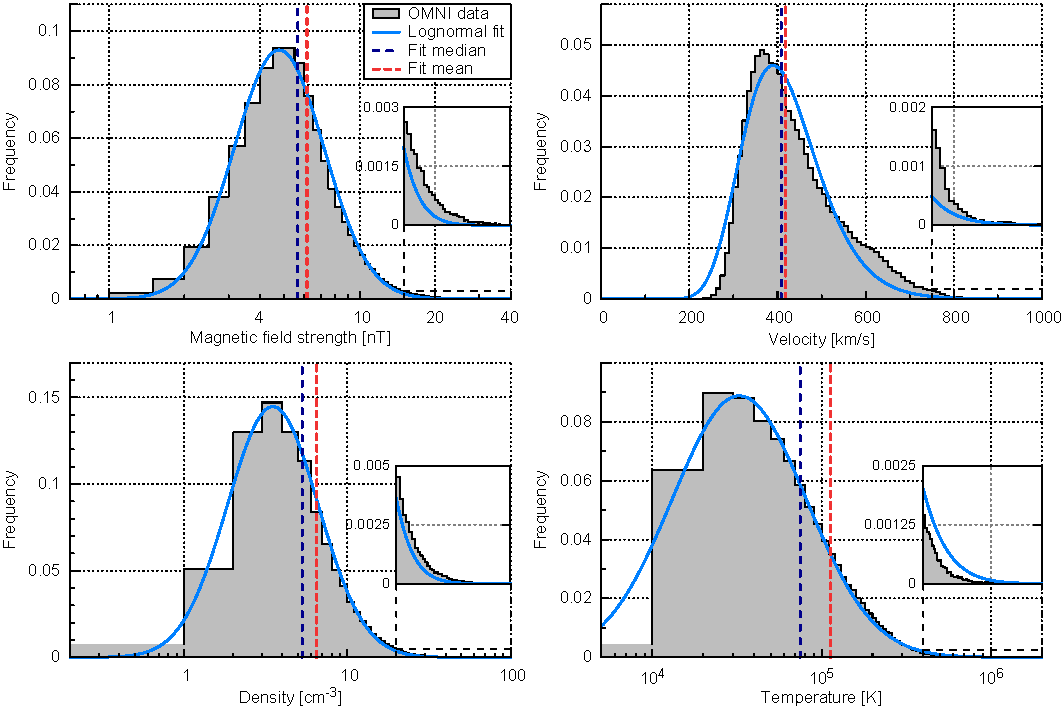
\includegraphics[width=18cm]{figures/histogram_fits_4_a_zoom_paper_pdfplot.pdf}
	\caption{Frequency distributions of the four solar wind parameters and their lognormal fits derived from the hourly OMNI data set. The histograms have bins of \SI{0.5}{\nT}, \SI{10}{\km\per\s}, \SI{1}{\per\cm\cubed} and \SI{10000}{\K}. The fits' median and mean values are indicated as well. The insets show zoomed-in frequency axes.}
	\label{fig:histogram_fits_4_a_zoom_paper_pdfplot}
\end{figure*}

%double lognormal fitting
%%%%%%%%%%%%%%%%%%%%%%%%%
%justification for compositional lognormal fit
In order to find a better fit result for the velocity distribution, we assume that the velocity distribution can be made up of at least two overlapping branches \citep{McGregor2011b}. Therefore a compositional approach  is chosen by combining two lognormal functions (\ref{eq:single_lognormal_fit_function}), involving more fit variables:
\begin{align}
	W_\text{II}(x) &= c \cdot W_1(x) + (1 -c) \cdot W_2(x)\,.	\label{eq:double_lognormal_fit_function}
\end{align}
The balancing parameter $c$ ensures that the resulting function remains normalized as it represents a probability distribution.
The fitting of $W_\text{II}(x)$ to the velocity's frequency distribution yields the values of the now five fit parameters ($c$, $x_\text{med,1}$, $x_\text{avg,1}$, $x_\text{med,2}$ and $x_\text{avg,2}$) as listed in Table~\ref{tab:lognormal_fit_parameters} together with the median and mean values of the composed distribution, which can be derived via solving
\begin{align}
	\int W_\text{II}(x)\,\text{d}x = 0	&	&\text{and}	&	&\int x\,W_\text{II}(x)\,\text{d}x = 0	\,.
\end{align}
This more complex fit function is more accurate in describing the velocity's frequency distribution as shown in Fig.~\ref{fig:histogram_fits_V_a_zoom_dbl_paper_pdfplot}.
\begin{figure}
	\resizebox{\hsize}{!}{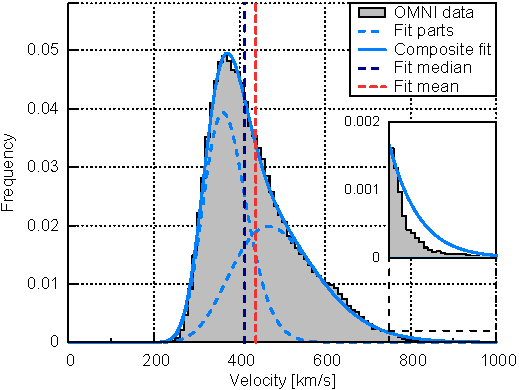
\includegraphics{figures/histogram_fits_V_a_zoom_dbl_paper_pdfplot.pdf}}
	\caption{The velocity's frequency distribution (same as in Fig.~\ref{fig:histogram_fits_4_a_zoom_paper_pdfplot}) and its compositional lognormal fit. The fit's median and mean values and its two fit parts are indicated as well. The inset has a zoomed-in frequency axis.}
	\label{fig:histogram_fits_V_a_zoom_dbl_paper_pdfplot}
\end{figure}
Thus in the following sections we keep the double lognormal ansatz for all velocity frequency fits.

%transition
For the bulk of the solar wind these static lognormal functions describe the parameters' distributions well, but differ for the extreme values, mainly caused by CME events.
The simple lognormal fit functions underestimate the frequency of the solar wind parameters in their high value tails, except for the temperature’s tail which is overestimated as seen in the insets of Fig.~\ref{fig:histogram_fits_4_a_zoom_paper_pdfplot}. The velocity's compositional lognormal fit only slightly overestimates its tail as seen in the inset of Fig.~\ref{fig:histogram_fits_V_a_zoom_dbl_paper_pdfplot}.
The slow and fast part contribute almost equally ($c \approx 0.5$) to the long-term velocity distribution function.

{\color{red} discuss high value zoom figures; read in Veselovsky2010}


\section{Solar activity dependence of the solar wind frequency distributions}
\label{sec:solar_activity_variations}
In the next step we investigate how the long-term solar wind distribution functions presented in the previous section depend on general solar activity. Therefore we examine their correlation with the sunspot number, being a commonly used long-term solar activity index, and determine the time lags with the highest correlation coefficients.

%\subsection{SSN data}
The international sunspot number (\citeyear{sidc}) is provided by the online catalogue\footnote{\url{http://www.sidc.be/silso/}} at the World Data Center -- Sunspot Index and Long-term Solar Observations (WDC-SILSO), Solar Influences Data Analysis Center (SIDC), Royal Observatory of Belgium (ROB).

%\subsection{SSN correlation}
For the correlations we fit lognormal functions to the frequency distributions as in Sect.~\ref{sec:frequency_distribution}, but implement linear relations to the yearly SSN, allowing shifting of the distribution functions with SSN. For the velocity the approach is different insofar as its two components are kept fixed and instead their balance is modified with the changing SSN.

Fig.~\ref{fig:OMNI_yearly_ssn_correlation_c_plot} shows yearly medians of the solar wind parameters and the yearly SSN together with the solar cycle number. The reason for correlating the SSN to the solar wind median values is because the position of a lognormal function is defined by its median. The data are averaged to yearly values to avoid seasonal effects during the Earth’s orbit around the Sun caused by its variations in solar latitude and distance.
\begin{figure}
	\resizebox{\hsize}{!}{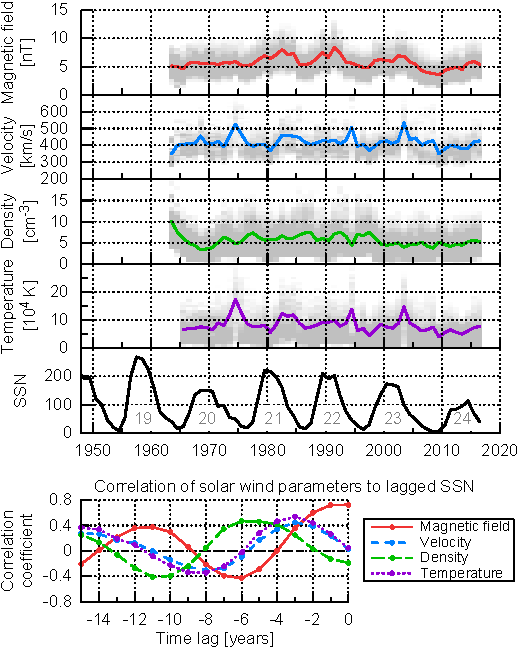
\includegraphics{figures/OMNI_yearly_ssn_correlation_c_plot.pdf}}
	\caption{The solar wind parameter yearly medians derived from OMNI data and the yearly SSN from the \citet{sidc} with solar cycle number (top). Their correlation coefficients with the yearly SSN are calculated for time lags back to -15 years (bottom).}
	\label{fig:OMNI_yearly_ssn_correlation_c_plot}
\end{figure}

The solar wind velocity, density and temperature depend on the state of the solar cycle \citep{Schwenn1983}. %density modulation with SSN \citep{Schwenn1983} p.~499\\
For instance the fast solar wind is correlated with the presence of polar coronal hole extensions to lower latitudes being a typical feature of the solar cycle, being the reason for the common velocity peak in the decreasing phase of the SSN, as pointed out by \citet[p.~75, Figure~3.52]{Bothmer2007}. Therefore the solar wind velocity, density and temperature maxima exhibit time-lags to the SSN maxima.

The correlation coefficients of the solar wind parameters with the yearly SSN shown in the bottom part of Fig.~\ref{fig:OMNI_yearly_ssn_correlation_c_plot} are calculated for time lags back to \num{-15}~years to cover a time span longer than a solar cycle. As expected, the correlation coefficients' amplitudes of all parameters decline with increasing time lag and show a frequency of about 11~years. The highest correlation coefficient of 0.728 to the SSN is found for the magnetic field strength, it has no time lag. This finding is anticipated because the SSN is found to be directly proportional to the evolution of the photospheric magnetic flux \citep{Smith2003}.
Velocity and temperature show a lag time of 3~years with peak correlation coefficients of 0.453 and 0.540. The density with a correlation coefficient of 0.468 has a time lag of 6~years, which is in agreement with the by \citet{Bougeret1984} reported density anticorrelation to the SSN.	%p.~406\\
% maximal correlation coefficients and their lag times:\\
% magnetic field strength: lag 0, 0.728\\
% velocity: lag -3, 0.453\\
% density: lag -6, 0.468\\
% temperature: lag -3, 0.540\\

%\subsection{SSN fitting}
To enable shifts of the solar wind frequency distributions with the SSN, we add a linear SSN dependency to the median
\begin{align}
	x_\text{med}(ssn) &= a_\text{med} \cdot ssn + b_\text{med}\,,	\label{eq:median_with_ssn}
\end{align}
using a factor to the SSN $a_\text{med}$ with a baseline $b_\text{med}$. We relate the mean with a scaling factor to the median to transfer its SSN dependency:
\begin{align}
	x_\text{avg}(ssn) &= (1 + a_\text{avg}) \cdot x_\text{med}(ssn)\,.	\label{eq:mean_with_ssn}
\end{align}
With the implementation of these relations into the lognormal function (\ref{eq:single_lognormal_fit_function}), the new dynamic fit function $W'(x,ssn)$ is then fitted to the yearly data. The three resulting fit coefficients ($a_\text{med}, b_\text{med}$ and $a_\text{avg}$) are presented in Table~\ref{tab:ssn_fit_parameters}.
\begin{table*}
	\caption{Resulting fit coefficients from the OMNI data fitting with lagged SSN. For the velocity the fit parameters from the double lognormal fit and their balancing function are given. The values in brackets are the estimated standard deviation of the fit parameters.}
	\label{tab:ssn_fit_parameters}
	\centering
	\begin{tabular}{l@{} c@{}
		S[table-format = 1.3(2)e+1]
		S[table-format = 1.4(2)]
		S[table-format = 1.3(2)e+1]
		S[table-format = +1.3(2)e+1]
		c
		}
		\hline\hline
		\multicolumn{2}{l}{\multirow{2}{*}{Parameter}}	&\multicolumn{2}{c}{Median\tablefootmark{a}}	&\multicolumn{1}{c}{Mean}	&\multicolumn{2}{c}{Balance}\\
		\cline{3-4}\cline{6-7}
		\multicolumn{2}{l}{}	&\multicolumn{1}{c}{SSN factor $a_\text{med}$}	&\multicolumn{1}{c}{Baseline $b_\text{med}$}	&\multicolumn{1}{c}{Scaling factor $a_\text{avg}$}	&\multicolumn{1}{c}{SSN factor $c_a$}	&\multicolumn{1}{c}{Baseline $c_b$}\\
		\hline
		\multicolumn{2}{l}{Magnetic field}	&1.309(19)e-2	&4.285(17)	&8.786(78)e-2	&\multicolumn{1}{c}{--}	&--\\
%		\multicolumn{2}{l}{Velocity}	&2.514(93)e-3	&3.8521(90)	&2.392(26)e-2	&\multicolumn{1}{c}{--}	&--\\
		\multicolumn{2}{l}{Density}	&3.81(25)e-3	&4.495(26)	&3.050(27)e-1	&\multicolumn{1}{c}{--}	&--\\
		\multicolumn{2}{l}{Temperature}	&1.974(26)e-2	&5.729(19)	&6.541(28)e-1	&\multicolumn{1}{c}{--}	&--\\
		\hline
		\multirow{2}{*}{Velocity}	&\multicolumn{1}{c}{$W'_1$}	&\multicolumn{1}{c}{--}	&3.633(12)	&1.008(37)e-2	&\multirow{2}{*}{\tablenum{-1.799(95)e-3}}	&\multirow{2}{*}{0.638(32)}\\
			&\multicolumn{1}{c}{$W'_2$}	&\multicolumn{1}{c}{--}	&4.831(81)	&2.31(20)e-2	&	&\\
		\hline
	\end{tabular}
	\tablefoot{
		\tablefoottext{a}{In units of \si{nT}, \SI{e2}{\km\per\s}, \si{\per\cm\cubed} and \SI{e4}{\K}.}
	}
\end{table*}

As can be seen from Fig.~\ref{fig:OMNI_yearly_BVdblNTSSN_fit_e_plot}, naturally, the fit models match with the general data trends, though single year variations are not replicated by the model (e.g., the high velocity and temperature values in 1974, 1994 and 2003).
\begin{figure*}
	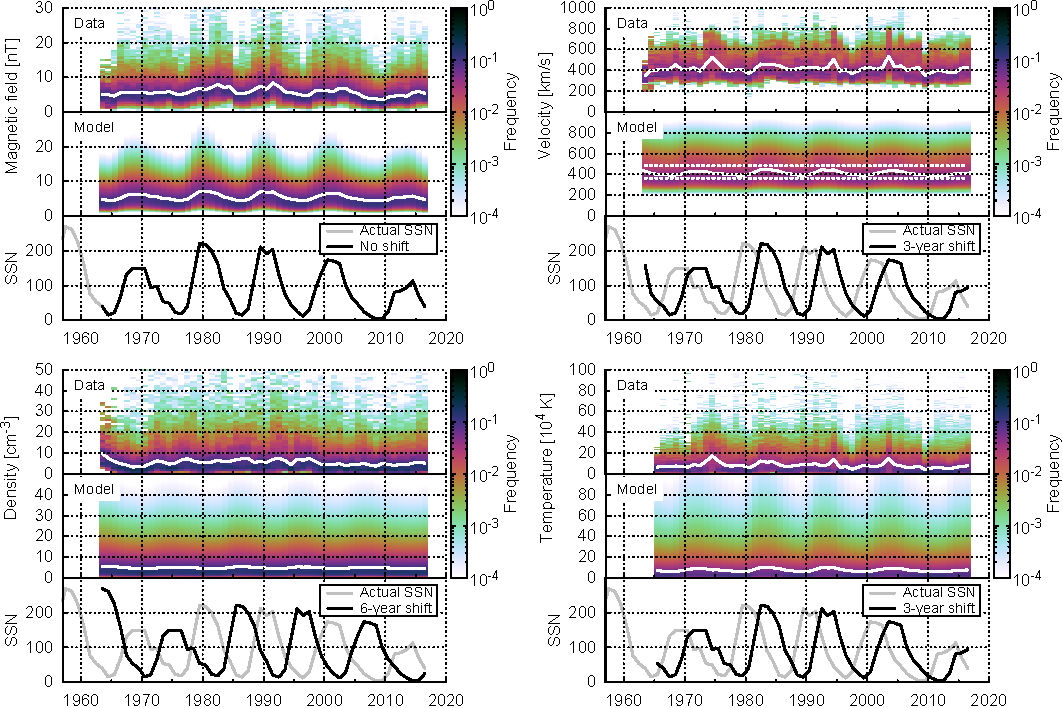
\includegraphics[width=18cm]{figures/OMNI_yearly_BVdblNTSSN_fit_e_plot.pdf}
	\caption{Solar wind parameter yearly data frequencies and lognormal fit models, both with their median values (white lines) over the OMNI time period 1963--2016. The corresponding yearly SSN and the for the models shifted SSN are indicated by grey and black lines. The velocity median is derived from the SSN weighted constant lognormal parts (dotted lines).}
	\label{fig:OMNI_yearly_BVdblNTSSN_fit_e_plot}
\end{figure*}
The comparison of this model with the yearly data median values with respect to the lagged SSN shows that the medians obtained from the modeling have a quite similar slope as shown in Fig.~\ref{fig:OMNI_yearly_BVNTvsSSN_a}.
\begin{figure}
	\resizebox{\hsize}{!}{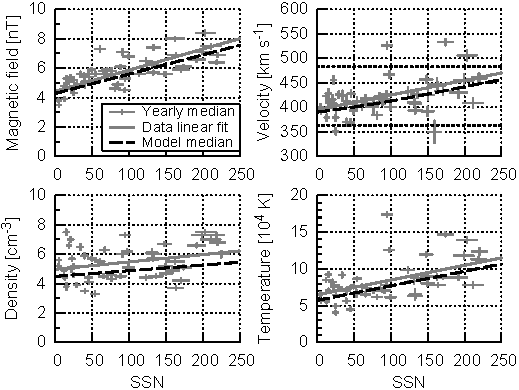
\includegraphics{figures/OMNI_yearly_BVNTvsSSN_a.pdf}}
	\caption{Solar wind parameter median with respect to the lagged SSN. The yearly data medians (+) with their weighted linear fit (solid lines) are obtained from OMNI data. The error bars denote the SSN standard deviation and the relative weight from the yearly data coverage. The SSN dependent median (\ref{eq:median_with_ssn}) is derived from the lognormal model fit (dashed line). For the velocity the median is derived from the SSN weighting (\ref{eq:balance_with_ssn}) of the slow and fast model parts, whose magnitudes are SSN independent (dotted line).}
	\label{fig:OMNI_yearly_BVNTvsSSN_a}
\end{figure}

Again, the solar wind velocity needs a special treatment because of the application of the double lognormal distribution (\ref{eq:double_lognormal_fit_function}). Since it is well known that slow and fast solar wind stream occurrence rates follow the solar cycle we keep the two velocity components' positions constant and vary instead their balance with the SSN:
\begin{align}
	c(ssn) &= c_a \cdot ssn + c_b\,.	\label{eq:balance_with_ssn}
\end{align}
The fit result (see Table~\ref{tab:ssn_fit_parameters}) yields a model in which three years after solar cycle minimum (SSN of zero) the contribution of slow solar wind to the overall solar wind distribution reaches a maximum value of about \SI{64}{\percent} and decreases with increasing SSN as shown in Fig.~\ref{fig:Vdbl_SSN_ratio_f_plot}.
\begin{figure}
	\resizebox{\hsize}{!}{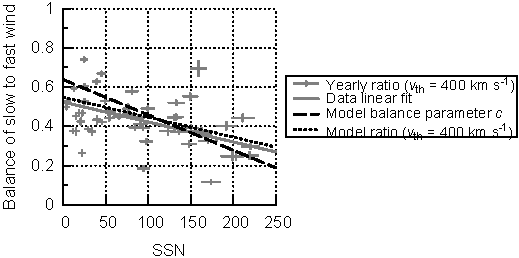
\includegraphics{figures/Vdbl_SSN_ratio_f_plot.pdf}}
	\caption{Ratio of slow to fast solar wind for a by 3~years lagged SSN. The yearly ratios (+) and their weighted linear fit (solid line) are obtained from OMNI data with a threshold velocity of $v_\text{th} = \SI{400}{\km\per\s}$. The error bars denote the SSN standard deviation and the relative weight from the yearly data coverage. The model's balance parameter (\ref{eq:balance_with_ssn}) and derived ratio (same threshold) are plotted as dashed and dotted lines.}
	\label{fig:Vdbl_SSN_ratio_f_plot}
\end{figure}
% 3 years after minimum (SSN of zero) the slow wind has its maximal share of 0.638(32). 3 years after maximum (SSN of 200) it has only a share of 0.278(37).

To investigate the amount of slow and fast wind contributions depending on solar activity, we apply the commonly used constant velocity threshold of $v_\text{th} = \SI{400}{\km\per\s}$ \citep[p.~144]{Schwenn1990}. The linear fit to the yearly data ratio and the derived model ratio show a good agreement (see Fig.~\ref{fig:Vdbl_SSN_ratio_f_plot}). Specific velocity thresholds between slow and fast solar wind cannot be directly compared with the to some degree steeper balance parameter of the double fit function used in this model. However, it appears being likely a more realistic approach than just taking a specific velocity threshold for the slow and fast wind, in agreement with the overlapping nature of the velocity flows reported by \citet{McGregor2011b}.
%(i.e. there exists slow wind with properties of fast wind and vice versa)


%exponential fitting
%%%%%%%%%%%%%%%%%%%%
\section{Solar distance dependency}
\label{sec:solar_distance_dependency}
In order to derive heliocentric distance relationships of the bulk solar wind distribution functions, we apply and fit a power law dependency to the Helios data. We evaluate the fits’ extrapolation behavior in direction to the Sun, because in a subsequent step it will be extrapolated to the PSP orbit. We use the fitting methods of Sect.~\ref{sec:frequency_distribution} for the distance-binned combined data from both Helios probes. Helios’ highly elliptical orbits in the ecliptic covered a solar distance range of \SIrange{0.31}{0.98}{\au} in case of Helios~1 and \SIrange{0.29}{0.98}{\au} in case of Helios~2. Launched during solar cycle minimum, the data of both probes cover the rise to the maximum of cycle~21, covering $\sim$6.5~years at varying distances to the Sun.

In the same way as the OMNI data we investigate hourly averages of the Helios data. The Helios~1 merged hourly data from the magnetometer and plasma instruments \citep{Rosenbauer1977} include $\sim$12.5~orbits for the time range 10~December 1974 until 14~June 1981, those for Helios~2 include $\sim$8~orbits for the time span 1~January 1976 until 4~March 1980. The data are retrieved from the Coordinated~Data~Analysis~Web (CDAWeb) interface at NASA's GSFC/SPDF\footnote{\url{http://spdf.gsfc.nasa.gov/}}.
%Helios plasma instrument (E1); Helios magnetometer instrument (E2)
% Helios data ranges:\\
% - time range Helios~1 [1974-12-10--1981-06-14] (12.5~orbits), Helios~2 [1976-01-01--1980-03-04] (8~orbits)\\
% - solar distance range Helios~1 0.31--0.98~au, Helios~2 0.29--0.98~au\\
%data sources

The Helios~1 magnetometer data coverage for this data set is about \SI{43}{\%} (i.e., 2.8~years), that of Helios~2 amounts to \SI{54}{\%} (i.e., 2.3~years). The plasma data coverage is \SI{76}{\%} (i.e., 5.0~years) in case of Helios~1 and \SI{92}{\%} (i.e., 3.9~years) in case of Helios~2. 
% temporal coverage of merged data\\
% Helios 1: 1974-12-10--1981-06-14; 6y6m15d = 2388~d = 6.538~y\\
% Mag data coverage: 42.6~\%; 2.785~years\\
% Plasma data coverage: 76.4~\%; 4.995~years\\
% Helios 2: 1976-01-01--1980-03-04; 4y3m4d = 1557~d = 4.263~y\\
% Mag data coverage: 54.4~\%; 2.319~years (83~\% of H1)\\
% Plasma data coverage: 91.8~\%; 3.913~years (78~\% of H1)\\
%Helios data biased towards solar minimum
Thus, using this data, one has to keep in mind that its time coverage is unequally distributed over the solar cycle. Considering the data gap distributions, the amount of data during solar cycle minimum up to mid~1977, that is, the transition from minimum to maximum, covers about \SI{68}{\percent} whereas during maximum of cycle~21 data are available only \SI{38}{\percent} of the time. This Helios data bias towards solar minimum is the reason why in this study the Helios solar wind data are not used to derive long-term frequency distributions and solar cycle dependencies for the key solar wind parameters.
% data gaps -> uneven coverage -> solar cycle minimum dominates; ratio of max vs min cycle data coverage; for OMNI data negligible\\
% 13~months smoothed sunspot number \citep{sidc}: divide June~1977 (include figure)\\
% put link on sidc webpage: http://sidc.be/sunspot-data/SIDCpub.php
% begin: 1974-12 36.1\\
% minimum: May/June 1976 18.3/17.9 (cite?)\\
% divide 30~June~1977 37.7 from SIDC data (nearly same SSN as at Helios~1 beginning)\\
% cycle 21 maximum: Dec 1979 232.9 (cite?)\\
% end: 1981-06 200.9\\
% 
% data gap hours and percentages:\\
% % H1 minimum 22416 h\\
% % H1 maximum 34681 h\\
% % H2 minimum 13128 h\\
% % H2 maximum 23472 h\\
% % sum 93697 h\\
% solar minimum: 35\,544~h, 37.94~\%\\
% solar maximum: 58\,153~h, 62.06~\%\\

% 1974 11 1974.874   39.3   4.2    30  
% 1974 12 1974.958   36.1   4.0    31  
% 1975 01 1975.042   33.0   3.9    31  
% 1975 02 1975.123   31.8   3.8    28  
% 1975 03 1975.204   30.6   3.7    31  
% 1975 04 1975.288   26.8   3.5    30  
% 1975 05 1975.371   24.2   3.3    31  
% 1975 06 1975.455   23.2   3.3    30  
% 1975 07 1975.538   21.8   3.2    31  
% 1975 08 1975.623   20.7   3.1    31  
% 1975 09 1975.707   20.9   3.1    30  
% 1975 10 1975.790   22.3   3.2    31  
% 1975 11 1975.874   23.3   3.3    30  
% 1975 12 1975.958   23.6   3.3    31  
% 1976 01 1976.042   22.1   3.2    31  
% 1976 02 1976.124   19.2   3.0    29  
% 1976 03 1976.206   17.8   2.9    31  
% 1976 04 1976.290   18.4   2.9    30  
% 1976 05 1976.373   18.3   2.9    31  
% 1976 06 1976.456   17.9   2.9    30  
% 1976 07 1976.540   18.8   2.9    31  
% 1976 08 1976.624   20.5   3.1    31  
% 1976 09 1976.708   20.8   3.1    30  
% 1976 10 1976.791   19.7   3.0    31  
% 1976 11 1976.874   19.7   3.0    30  
% 1976 12 1976.958   21.6   3.2    31  
% 1977 01 1977.042   24.3   3.3    31  
% 1977 02 1977.123   26.3   3.5    28  
% 1977 03 1977.204   28.8   3.6    31  
% 1977 04 1977.288   31.9   3.8    30  
% 1977 05 1977.371   34.7   4.0    31  
% 1977 06 1977.455   37.7   4.1    30  
% 1977 07 1977.538   41.4   4.3    31  
% 1977 08 1977.623   47.6   4.6    31  
% 1977 09 1977.707   55.8   5.0    30  
% 1977 10 1977.790   64.8   5.4    31  
% 1977 11 1977.874   73.7   5.7    30  
% 1977 12 1977.958   80.7   6.0    31  
% 1978 01 1978.042   86.9   6.2    31  
% 1978 02 1978.123   91.5   6.4    28  
% 1978 03 1978.204   98.7   6.6    31  
% 1978 04 1978.288  109.0   7.0    30  
% 1978 05 1978.371  117.8   7.2    31  
% 1978 06 1978.455  126.6   7.5    30  
% 1978 07 1978.538  138.0   7.8    31  
% 1978 08 1978.623  147.3   8.1    31  
% 1978 09 1978.707  153.6   8.3    30  
% 1978 10 1978.790  157.3   8.4    31  
% 1978 11 1978.874  160.4   8.5    30  
% 1978 12 1978.958  166.7   8.6    31  
% 1979 01 1979.042  175.2   8.8    31  
% 1979 02 1979.123  185.4   9.1    28  
% 1979 03 1979.204  193.3   9.3    31  
% 1979 04 1979.288  199.9   9.4    30  
% 1979 05 1979.371  208.5   9.6    31  
% 1979 06 1979.455  216.7   9.8    30  
% 1979 07 1979.538  219.5   9.9    31  
% 1979 08 1979.623  220.1   9.9    31  
% 1979 09 1979.707  220.4   9.9    30  
% 1979 10 1979.790  223.4  10.0    31  
% 1979 11 1979.874  229.8  10.1    30  
% 1979 12 1979.958  232.9  10.2    31  
% 1980 01 1980.042  232.0  10.2    31  
% 1980 02 1980.124  230.2  10.2    29  
% 1980 03 1980.206  227.9  10.1    31  
% 1980 04 1980.290  224.6  10.0    30  
% 1980 05 1980.373  221.3  10.0    31  
% 1980 06 1980.456  219.1   9.9    30  
% 1980 07 1980.540  216.1   9.9    31  
% 1980 08 1980.624  212.0  10.0    31  
% 1980 09 1980.708  211.5  10.2    30  
% 1980 10 1980.791  211.9  10.5    31  
% 1980 11 1980.874  209.1  10.9    30  
% 1980 12 1980.958  202.8  11.0    31  
% 1981 01 1981.042  199.6  11.1   271  
% 1981 02 1981.123  202.2  11.5   229  
% 1981 03 1981.204  205.4  12.1   244  
% 1981 04 1981.288  205.7  12.6   254  
% 1981 05 1981.371  204.1  12.8   268  
% 1981 06 1981.455  200.9  13.1   227  
% 1981 07 1981.538  198.5  13.1   268  

The median and mean values of the key solar wind parameters for different solar distances of the Helios data are calculated for the minimal distance resolution \SI{0.01}{\au} of the data set, see Fig.~\ref{fig:radial_fit_4_thesis_light_skip_pdfcairo_plot}. Assuming a radial solar wind outflow, it is expected that the distance dependence of the solar wind parameters over the Helios data range \SIrange{0.29}{0.98}{\au} can be described through power law scaling. Therefore we use the power law function
\begin{align}
	x(r) = d\cdot r^e	\label{eq:power_function}
\end{align}
for the regression fit of the median and mean, with $r$ being the solar distance in astronomical units, $d$ the magnitude at \SI{1}{\au} and $e$ the exponent. The fits are weighted through the different data counts per bin.
%fit result table and figure
The fit coefficients ($d_\text{med}$, $d_\text{avg}$, $e_\text{med}$ and $e_\text{avg}$) are listed in Table~\ref{tab:mean_median_fit_parameter}.
\begin{table*}
	\caption{Fit coefficients for the median and mean solar distance dependencies of the four solar wind parameters derived from the combined Helios~1 and 2 data. The errors in brackets are the estimated standard deviations of each fit parameter. The crossing distances indicate where the median and mean fits intersect each other. The yearly variation is the weighted standard deviation derived from the yearly fit exponents seen in Fig.~\ref{fig:yearly_gradients_c}.}
	\label{tab:mean_median_fit_parameter}
	\centering
	\begin{tabular}{l
	S[table-format = 1.3(2)]
	S[table-format = +1.3(2)]
	@{}c
	S[table-format = 1.3(2)]
	S[table-format = +1.3(2)]
	S[table-format = 1.1(2)e1]
	S[table-format = 1.3]}
		\hline\hline
		\multirow{2}{*}{Parameter}	&\multicolumn{2}{c}{Median}	&	&\multicolumn{2}{c}{Mean}	&\multicolumn{1}{c}{Crossing distance}	&\multicolumn{1}{c}{Yearly variation}\\
		\cline{2-3}	\cline{5-6}
			&\multicolumn{1}{c}{$d_\text{med}$\tablefootmark{a}}	&\multicolumn{1}{c}{$e_\text{med}$}	&	&\multicolumn{1}{c}{$d_\text{avg}$\tablefootmark{a}}	&\multicolumn{1}{c}{$e_\text{avg}$}	&\multicolumn{1}{c}{[\si{\au}]}	&\multicolumn{1}{c}{$\Delta e$}\\
		\hline
		Magnetic field	&5.377(92)	&-1.655(17)	&	&6.05(10)	&-1.546(18)	&0.339(11)	&0.11\\
		Velocity	&4.107(28)	&0.058(13)	&	&4.356(24)	&0.049(10)	&0.7(83)e3	&0.012\\
		Density		&5.61(27)	&-2.093(46)	&	&7.57(30)	&-2.010(38)	&0.027(73)	&0.072\\
		Temperature	&7.14(23)	&-0.913(39)	&	&9.67(21)	&-0.792(28)	&0.082(85)	&0.005\\
		\hline
	\end{tabular}
	\tablefoot{
		\tablefoottext{a}{In units of \si{nT}, \SI{e2}{\km\per\s}, \si{\per\cm\cubed} and \SI{e4}{\K}.}
	}
\end{table*}
% source year variation: fit_out_yearly_gradients_table_b_stats.txt

% comparison with other Helios studies (Schwenn, Bougeret)
%Helios results, radial gradients see \citet{Schwenn1990} p.~155
As anticipated, our derived exponents agree with those found in existing studies from the Helios observations: \citet{Mariani1978} derived the exponents for the magnetic field strength separately for the fast and the slow solar wind as $B_\text{fast} \propto r^{-1.54}$ and $B_\text{slow} \propto r^{-1.61}$.
%$B_\text{fast} = 5.79\cdot r^{-1.54}$\,nT and $B_\text{slow} = 5.11\cdot r^{-1.61}$\,nT.
The velocity exponent matches with the values found by \citet{Schwenn1983,Schwenn1990}, who derived the distance dependencies for both Helios spacecraft separately as $v_\text{H1} \propto r^{0.083}$ and $v_\text{H2} \propto r^{0.036}$. The calculated density exponent agrees well with the Helios plasma density model derived by \citet{Bougeret1984}, yielding $n \propto r^{-2.10}$.
%to the year 1976 normalized   a \SI{1}{\au} density of $n = 6.14\cdot r^{-2.10}\,\text{cm}^{-3}$.
The temperature exponent is similar to those in the studies by \citet{Hellinger2011,Hellinger2013}, who also derived the exponents separately for the fast and the slow solar wind: $T_\text{fast} \propto r^{-0.74}$ and $T_\text{slow} \propto r^{-0.58}$.
%$T_\text{fast} = \num{2.5e5} (R/R_0)^{-0.74}$\,K and $T_\text{slow} = \num{6.2e4} (R/R_0)^{-0.58}$\,K.
%\citet{Marsch1982}	$T_\text{||,slow} \propto r^{-1.03}$ and $T_\text{||,fast} \propto r^{-0.69}$.


%crossing distances
Fig.~\ref{fig:radial_fit_4_thesis_light_skip_pdfcairo_plot} shows the radial dependence of the solar wind parameters over the distance range \SIrange{0.29}{0.98}{\au} and the mean and median values and their respective power law fits. The mean and median velocity fit exponents are very similar, which indicates that they just as well can be kept identical so that the basic shape of the frequency distribution does not change with distance.
\begin{figure*}
	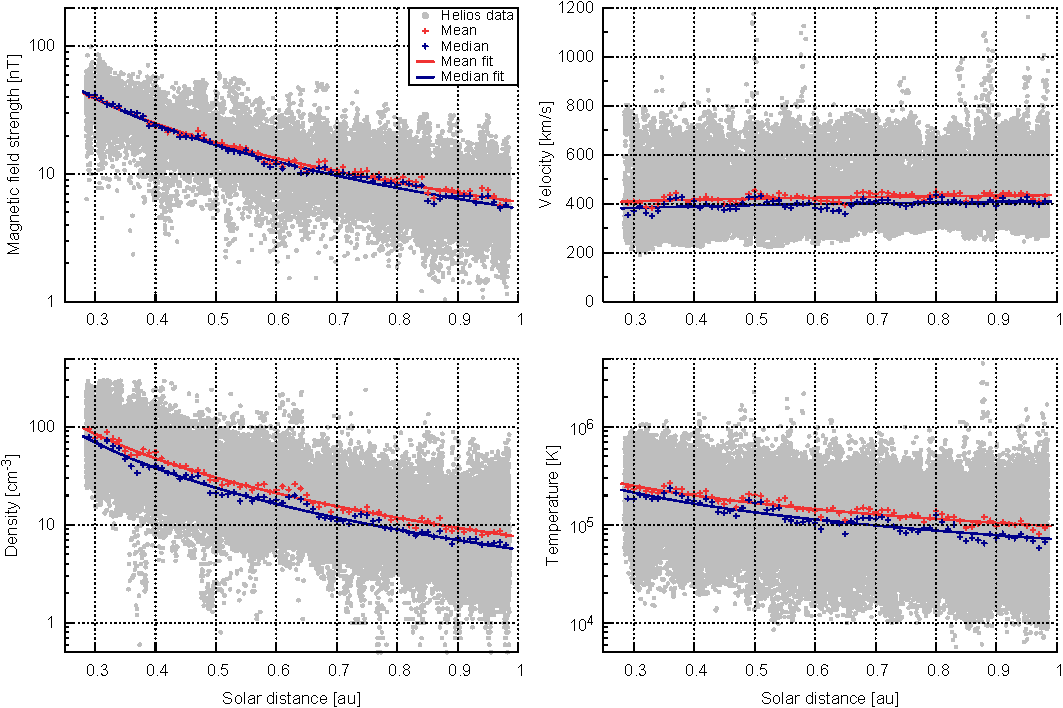
\includegraphics[width=18cm]{figures/radial_fit_4_thesis_light_skip_pdfcairo_plot.pdf}
	\caption{Helios hourly data plots of the four solar wind parameters over solar distance. The mean and median per \SI{0.01}{\au} data bin and their fit curves are plotted as well. The Helios data has a native distance resolution of \SI{0.01}{\au}, thus, to make the abundance visible in these plots, we added a random distance value of up to \SI{+-0.005}{\au}.}
	\label{fig:radial_fit_4_thesis_light_skip_pdfcairo_plot}
\end{figure*}
Contrary, the mean and median fits for the magnetic field strength cross each other at \SI{0.339}{\au} and the mean is lower than the median at smaller distances (Table~\ref{tab:mean_median_fit_parameter}). Thus, below that distance the distribution function cannot well be described anymore by a lognormal function. The fits for the proton temperature show a similar behavior,
having an intersection at \SI{0.082}{\au}. Therefore the extrapolation of the magnetic field and temperature distribution frequencies to the PSP orbit by applying lognormal functions is limited. To circumvent such limitations we set the exponents $e_\text{med}$ and $e_\text{avg}$ to be identical for all four parameters. It should be noted that this simplification leads to slightly larger modeling errors, especially in case of the magnetic field strength.

%\subsection{Power law lognormal fitting}
Next we retrieve the frequency distributions of the four parameters in distance bins of \SI{0.01}{\au},  choosing the same resolution as for the OMNI data analyzed in Sect.~\ref{sec:frequency_distribution}---the distributions are plotted in Fig.~\ref{fig:mixed_fit_fixed_4_paper_f_plot}.
% Helios histogram bin sizes for mean of frequency distribution (at specific solar distance):\\
% $B$: bin size 0.5~nT, min 337, mean precision: 0.000545\\
% $v$: bin size 1~cm$^{-3}$, min 497, mean precision: 0.00449\\
% $n$: bin size 10~km/s, min 497, mean precision:  0.00449\\
% $T$: bin size 10\,000~K, min 497, mean precision: 4.49--44.49\\
For simplification, as mentioned before, we treat the exponents of the median and mean fit functions as being identical. Implementing the power law distance dependency~(\ref{eq:power_function}) into the lognormal function (\ref{eq:single_lognormal_fit_function}), we get the fit parameters ($d'_\text{med}$, $d'_\text{avg}$ and their common exponent $e'$). Again, we use the double lognormal function~(\ref{eq:double_lognormal_fit_function}) for the velocity distribution fit, resulting in $W''_\text{II}(x,r)$. The additional fit parameters are the balancing parameter $c'$ and for the second lognormal part $d'_\text{med,2}$ and $d'_\text{avg,2}$. The resulting fit coefficients for the four solar wind parameters are presented in Table~\ref{tab:extrapolation_model_fit_parameters}.
\begin{table*}
	\caption{Fit coefficients from the single lognormal power function, respectively double lognormal for the velocity from the combined Helios data. The errors in brackets are the estimated standard deviations of the fit parameters.}
	\label{tab:extrapolation_model_fit_parameters}
	\centering
	\sisetup{table-figures-integer=1, table-figures-decimal=3, table-figures-exponent=0}
	\begin{tabular}{l c
	S[table-format = 1.3(2), table-space-text-post = a, table-align-text-post = false]
	S[table-format = 1.3(2), table-space-text-post = a, table-align-text-post = false]
	S[table-format = +1.4(2)]
	S[table-format = 1.3(2)]}
		\hline\hline
		\multicolumn{2}{l}{\multirow{2}{*}{Parameter}}	&\multicolumn{1}{c}{Median\tablefootmark{a}}	&\multicolumn{1}{c}{Mean\tablefootmark{a}}	&\multicolumn{1}{c}{Exponent}	&\multicolumn{1}{c}{Balance}\\
			&	&\multicolumn{1}{c}{$d'_\text{med}$}	&\multicolumn{1}{c}{$d'_\text{avg}$}	&\multicolumn{1}{c}{$e'$}	&$c'$\\
		\hline
		\multicolumn{2}{l}{Magnetic field}	&5.358(25)	&5.705(28)	&-1.662(11)	&\multicolumn{1}{c}{--}\\
		\multicolumn{2}{l}{Density}	&5.424(33)	&6.845(47)	&-2.114(20)	&\multicolumn{1}{c}{--}\\
		\multicolumn{2}{l}{Temperature}	&6.357(64)	&10.72(14)	&-1.100(20)	&\multicolumn{1}{c}{--}\\
		\hline
		\multirow{1}{*}{Velocity}	&$W''_1$	&3.707(13)	&3.748(16)	&\multirow{2}{*}{0.0990(51)}	&\multirow{2}{*}{0.557(45)}\\
			&$W''_2$	&5.26(13)	&5.42(11)	&	&\\
		\cline{2-6}
		\multicolumn{2}{r}{$W''_\text{II}$}	&4.13(13)\tablefootmark{b}	&4.47(11)\tablefootmark{b}	&\multicolumn{1}{c}{--}	&\multicolumn{1}{c}{--}\\
		\hline
	\end{tabular}
	\tablefoot{
		\tablefoottext{a}{In units of \si{nT}, \SI{e2}{\km\per\s}, \si{\per\cm\cubed} and \SI{e4}{\K}.}
		\tablefoottext{b}{Velocity median and mean \SI{1}{\au} values for the resulting function. Error estimates derived from the individual fit part errors.}
	}
\end{table*}
% Vdbl fit:
% medians = 370.7, 526
% means = 374.8, 542
% c = 0.557
% via calculate_twolognormal_median.py:
% mean = 446.64
% median = 413.33

The velocity balancing parameter $c' = 0.557$ is in good agreement with the results for the SSN dependency (\ref{eq:balance_with_ssn}), because with a mean SSN of 59 during the Helios time period, $c(59) = 0.53$, as can be seen from Fig.~\ref{fig:Vdbl_SSN_ratio_f_plot}.

The frequency distribution data for the four solar wind parameters with respect to the radial distance from the Sun are plotted in Fig.~\ref{fig:mixed_fit_fixed_4_paper_f_plot}, together with their power law lognormal fits and the double lognormal fit for the velocity with their median values.
\begin{figure*}
	\includegraphics[width=18cm]{figures/mixed_fit_fixed_4_paper_f_plot.pdf}
	\caption{Frequency distributions of the four solar wind parameters with respect to the solar distance. Plotted are the binned Helios data and the power law lognormal fit models with their median values (white lines). The double lognormal model is used for the velocity, its slow and fast parts are indicated by dotted lines.}
	\label{fig:mixed_fit_fixed_4_paper_f_plot}
\end{figure*}
The model’s magnetic field strength is broader around values of \SI{40}{nT} at the lower distance boundary than the data's frequency distribution implies. This behavior is expected because of the distance independent shape approximation applied. The velocity and temperature models’ upper values show a higher abundance than the actual data, see also zoom boxes in Figs.~\ref{fig:histogram_fits_4_a_zoom_paper_pdfplot} and \ref{fig:histogram_fits_V_a_zoom_dbl_paper_pdfplot}.


\section{Empirical solar wind model}
\label{sec:empirical_solar_wind_model}
In order to estimate the solar wind environment for the PSP orbit, we combine the results from the solar wind frequency distributions’ solar activity relationships and their distance dependencies derived from the OMNI and Helios data. The result is an empirical solar wind model for the inner heliosphere which will then be extrapolated to the PSP orbit in Sec.~\ref{sec:model_extrapolation_to_psp_orbit}.

%\subsection{Distance scaling law variations}
%\label{sec:distance_scaling_law_variations}
This established solar wind model for the radial distance dependence is representative for the time of the Helios observations around the rise of solar cycle~21. The variation of yearly power law fit exponents are shown in Fig.~\ref{fig:yearly_gradients_c} together with the yearly SSN for the time period \numrange{1974}{1982}. It can be seen that during the Helios time period there might be some systematic  variation of the exponents with solar activity---at least for the velocity and temperature. exponents
\begin{figure}
	\resizebox{\hsize}{!}{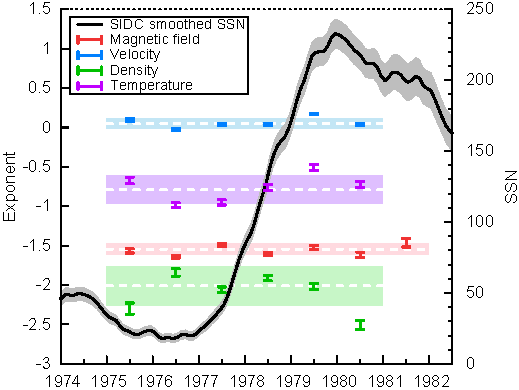
\includegraphics{figures/yearly_gradients_c.pdf}}
	\caption{Helios yearly variation of the solar wind parameters' fit exponents together with the SIDC 13-month smoothed monthly SSN. The weighted standard deviations and average values for all years are indicated by the shaded areas. In this plot the 21~days since Helios launch in the year 1974 are omitted because a distance range of merely \SIrange{0.95}{0.98}{\au} was covered that year.}
	\label{fig:yearly_gradients_c}
\end{figure}
%yearly variation of the solar wind parameters' average fit function exponents
However, for simplicity we assume, that the distance scaling laws can be treated as time independent and include the calculated exponents’ yearly variations $\Delta e$, summarized in Table~\ref{tab:mean_median_fit_parameter}, as relative uncertainties.

Since we neglect possible variations of the distance scaling laws, we combine the frequency distribution’s median solar activity dependency (\ref{eq:median_with_ssn}) derived for \SI{1}{\au} from the OMNI data with the power law exponents (\ref{eq:power_function}) derived from the Helios data:
\begin{align}
	x_\text{med}(ssn,r) &= (a_\text{med} \cdot ssn + b_\text{med}) \cdot r^{e'}	\,.	\label{eq:general_sw_model}
\end{align}
Thus we obtain the combined model function $W'''(x,ssn,r)$ and for the velocity $W_\text{II}'''(x,ssn,r)$ with the double lognormal function (\ref{eq:double_lognormal_fit_function}).


\section{Model extrapolation to PSP orbit}
\label{sec:model_extrapolation_to_psp_orbit}
To estimate PSP’s solar wind environment during its mission time for its orbital positions, SSN predictions are included into the in the previous sections derived empirical solar wind model and extrapolations down to the PSP perihelion region are performed.

%\subsection{Near-Sun extrapolation for PSP orbit}
%PSP orbit
Parker Solar Probe is planned to launch in mid 2018. With its first Venus flyby it will swing into Venus' orbital plane, reaching already 93~days after launch in November 2018 a first perihelion with a distance of \SI{0.16}{\au}. Seven additional Venus flybys allow to finally reduce its perihelion distance to a minimum of \SI{9.86}{\Rs} \citep{Fox2015} as plotted in Fig.~\ref{fig:SPP_orbit_predicted_SSN_overview_e_plot}.

We extrapolate the derived empirical solar wind model (\ref{eq:general_sw_model}) to PSP’s orbital distance range and compare the results with those from the existing models shown in Fig.~\ref{fig:sw_extrapolation_ssn_b_plot}.
\begin{figure*}
	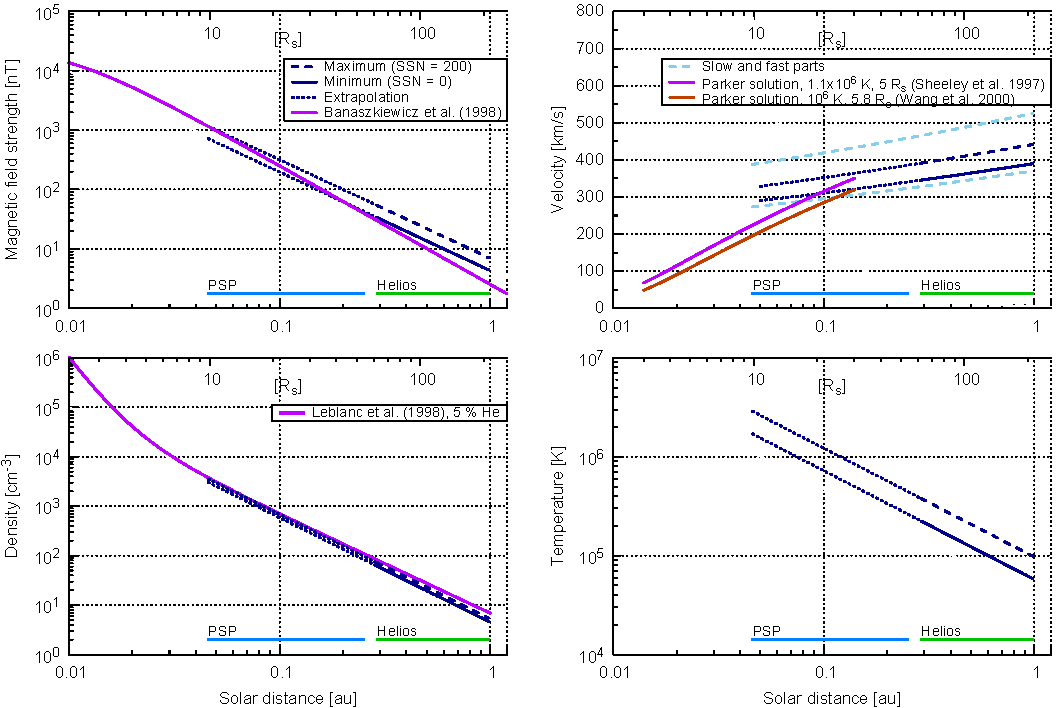
\includegraphics[width=18cm]{figures/sw_extrapolation_ssn_b_plot.pdf}
	\caption{Radial extrapolation of the solar wind parameters to the PSP orbit region. The from Helios and OMNI measurements obtained models are extrapolated to the PSP region---for the extreme cases of solar minimum (SSN = 0) and maximum (SSN = 200). Note that there is a time lag to the SSN depending on the solar wind parameter. The magnetic field radial dependence is slightly flatter than the analytic DQCS model for solar minimum which \citet{Banaszkiewicz1998} derived. \hl{Below} \SI{20}{\Rs} the slow wind velocity is overestimated in comparison to the measurements from \citet{Wang2000}) and \citet{Sheeley1997}. Down to PSP's perihelion the density is in good agreement with the model from \citet{Leblanc1998}. to 1-column...?}
	\label{fig:sw_extrapolation_ssn_b_plot}
\end{figure*}

%magnetic field:
The magnetic field strength is found to increase from median values of about \SI{43}{\nT} at \SI{0.25}{\au} to \SI{715}{\nT} at \SI{0.046}{\au} for a SSN of 0. Taking a SSN of 200 increases the value to \SI{69}{\nT} at \SI{0.25}{\au} and \SI{1152}{\nT} at \SI{0.046}{\au}. Our extrapolation results are slightly flatter than those derived from the analytical magnetic field model by \citet{Banaszkiewicz1998}, who constructed a dipole plus quadrupole plus current sheet (DQCS) model.
This difference is arguably due to the previously mentioned (Sect.~\ref{sec:solar_distance_dependency}) with solar distance changing shape of the frequency distribution, which for smaller distances deviates more from the model’s lognormal distribution.

%velocity:
The average velocity is found to decrease from \SI{340}{\km\per\s} at \SI{0.25}{\au} to about \SI{290}{\km\per\s} at \SI{0.046}{\au} for a SSN of 0. Whereas using a SSN of 200 it decreases from \SI{390}{\km\per\s} to \SI{330}{\km\per\s}. Comparing the results with those found by \citet{Sheeley1997} and \citet{Wang2000} shows an overestimation in our extrapolated velocity values for distances \hl{below} \SI{20}{\Rs}. They used LASCO coronagraph observations to track moving coronal features (blobs) in the distance range \SIrange{2}{30}{\Rs} to determine speed profiles and sources of the slow solar wind and they derived temperature and sonic point values for slow solar wind with the isothermal expansion model \citep{Parker1958}. Therefore, it generally can be expected that PSP will encounter a slower solar wind environment close to the Sun than our model estimates and thus PSP will measure solar wind acceleration processes \hl{below} \SI{30}{\Rs} \citep{Sheeley1997,McComas2008}.

%density:
The proton density increases from about \SI{84}{\per\cm\cubed} at  \SI{0.25}{\au} to about \SI{3018}{\per\cm\cubed} at \SI{0.046}{\au} for a SSN of 0. Being almost independent of the SSN the values for a SSN of 200 are only \SI{17}{\%} larger. The results are in good agreement with those of \citet{Leblanc1998}, who derived an electron density model from type~III radio burst observations. Their model shows that the density distance dependency scales with $r^{-2}$ and steepens just below \SI{10}{\Rs} with $r^{-6}$. For the comparison we assumed a solar wind helium abundance of \SI{5}{\%}.

%temperature:
The extrapolated proton temperature increases from about \SI{260000}{\K} at \SI{0.25}{\au} to about \SI{1690000}{\K} at \SI{0.046}{\au} for a SSN of 0 and from \SI{440000}{\K} to \SI{2860000}{\K} for a SSN of 200. Knowing that near-Sun coronal temperatures are in the range of \SIrange{2}{3}{\mega\K} \citep{Billings1959,Liebenberg1975}, the model \hl{may overestimate} the extrapolated temperatures at the PSP perihelion distance. {\color{red} The results can be compared to...}

%\subsection{SSN prediction for PSP mission time}
%SSN prediction
For SSN short-term predictions several sources are available. The SIDC provides 12-month SSN forecasts\footnote{\url{http://sidc.be/silso/forecasts}} obtained from different methods (e.g., Kalman filter combined method). The SSN prediction of NOAA's Space Weather Prediction Center (SWPC) follows for the time period until end of 2019 a consensus of the Solar~Cycle~24 Prediction~Panel\footnote{\url{http://www.swpc.noaa.gov/products/solar-cycle-progression}}.
For the prediction of the next solar cycle we simply assume a pattern similar to the last cycle and thus shift the last cycle by 11~years. Additionally we consider as possible alternatives SSN patterns of half and twice its amplitude as shown in Fig.~\ref{fig:SPP_orbit_predicted_SSN_overview_e_plot}.
The SSN for PSP's first perihelion will be small---certainly below 20, whereas PSP’s closest perihelia, which commence at the maximum phase of cycle~25 end of 2024, will experience as of now incalculable SSN amplitudes.
\begin{figure}
	\resizebox{\hsize}{!}{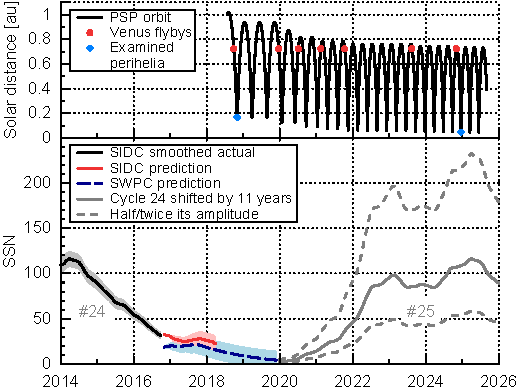
\includegraphics{figures/SPP_orbit_predicted_SSN_overview_e_plot.pdf}}
	\caption{PSP's solar distance during its mission time (top). Consecutive Venus flybys bring its perihelia nearer to the Sun. Actual and predicted SSN (bottom), that is, SIDC 13-month smoothed monthly actual SSN, SIDC prediction, SWPC prediction and by 11~years shifted SSN from previous cycle~24, together with two alternative trends of half and twice its amplitude.}
	\label{fig:SPP_orbit_predicted_SSN_overview_e_plot}
\end{figure}

%\subsection{PSP solar wind environment estimation}
Implementing the predicted SSN for the PSP mission time and the orbital trajectory data, we can finally derive the estimated solar wind environment $W'''(x,ssn,r)$, to infer which solar wind parameter magnitudes can be expected.

Figs.~\ref{fig:SPP_perihelia_prediction_e_plot} and \ref{fig:SPP_perihelia_prediction_nearest_e_plot} show the considered different solar wind parameters for 12-day periods, comprising the first perihelion in Novemver 2018 and the closest perihelion in December 2024. In the beginning of the mission peak median values of about \SI{87}{\nT}, \SI{340}{\km\per\s}, \SI{4015}{\per\cm\cubed} and \SI{503000}{\K} are estimated to be measured at \SI{0.16}{\au}, increasing to about \SI{943}{\nT}, \SI{290}{\km\per\s}, \SI{9733}{\per\cm\cubed} and \SI{1930000}{\K} during the closest approach at \SI{0.046}{\au}.
\begin{figure}
	\resizebox{\hsize}{!}{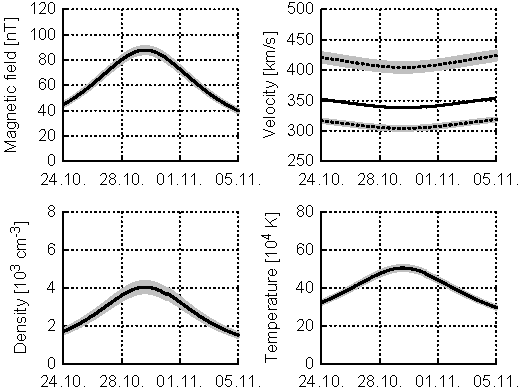
\includegraphics{figures/SPP_perihelia_prediction_e_plot.pdf}}
	\caption{Estimated solar wind parameter medians (black lines) and their error bands (grey) during 12 days in 2018 with PSP's first perihelion at about \SI{0.16}{\au}. For the velocity the combined median is calculated and also the SSN independent slow and fast parts are plotted (dotted lines).}
	\label{fig:SPP_perihelia_prediction_e_plot}
\end{figure}
\begin{figure}
	\resizebox{\hsize}{!}{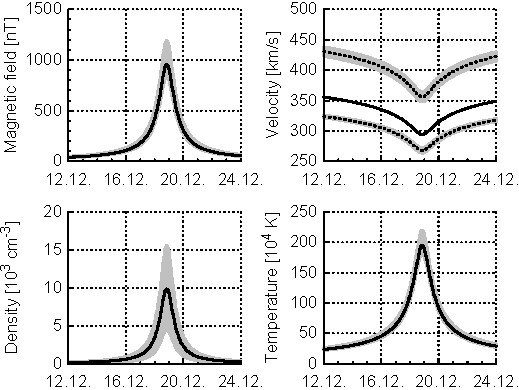
\includegraphics{figures/SPP_perihelia_prediction_nearest_e_plot.pdf}}
	\caption{Estimated solar wind parameter medians (black lines) and their error bands (grey) during during 12 days in 2024 with PSP's nearest perihelion at \SI{0.0459}{\au}. For the velocity the combined median is calculated and also the SSN independent slow and fast parts are plotted (dotted lines).}
	\label{fig:SPP_perihelia_prediction_nearest_e_plot}
\end{figure}


\section{Discussion}
\label{sec:discussion}

We started the development of the empirical solar wind environment model for the near-ecliptic PSP orbit by lognormally fitting the about 40~years of in situ near-Earth solar wind data collected in the OMNI database, using the frequency distributions of the key solar wind parameters magnetic field strength, velocity, density and temperature. The OMNI multi-satellite solar wind data is intercalibrated, covers almost five solar cycles and thus represents solar wind gathered at different phases of solar activity in the ecliptic plane. In the next step we investigated the yearly variation of the solar wind distribution functions along with the SSN over 53~years and derived linear dependencies of the solar wind parameters with the SSN. The radial dependencies of the solar wind distribution functions were then analyzed using Helios~1 and 2 data for the distance range \SIrange{0.29}{0.98}{\au} in bins of \SI{0.01}{\au}. The herefrom derived power law fit functions were used to scale the prior calculated SSN-dependent \SI{1}{\au} distribution fit functions to the PSP orbit, combined with SSN predictions for the years 2018--2025, i.e., for the prime mission phase that gets PSP to closest perihelia of 9.86~solar radii distance to the Sun. The reason for performing the analysis this way is based on the fact that the OMNI solar wind database is much larger than the Helios database. Though, it is clear that the calculated distribution functions just represent first order estimates of the real solar wind to be encountered by PSP. The solar wind environment to be encountered will depend at times of PSP on the structure of the solar corona and underlying photospheric magnetic field {\color{red} , as shown by \hl{xxx (ref.)},} and on the evolution and interaction of individual solar wind streams and superimposed CMEs and shocks.

However, the derived results are in good agreement with existing studies about near-Sun solar wind magnetic field strenghts and densities as shown in Sect.~\ref{sec:model_extrapolation_to_psp_orbit}. The from direct measurements differing velocity and temperature extrapolations below \hl{20~solar radii} indicate that PSP will indeed dive into the acceleration and heating regions of the solar wind to be expected at these distances (see Fig.~\ref{fig:sw_extrapolation_ssn_b_plot}). The near-Sun solar wind velocity at PSP perihelion is also expected to be slower than our model estimates, because the region of the Alfvénic critical surface, up to which the solar wind is believed to be accelerated, is predicted to lie in average around \SI{17}{\Rs} \citep[e.g.,][]{Sittler1999,Exarhos2000} and correlates with solar activity between \SI{15}{\Rs} in minimum and \SI{30}{\Rs} in maximum \citep{Katsikas2010,Goelzer2014}.	% in average around 17~Rs (e.g., 0.6~Rs Schatten 1969, 17~Rs Sittler1999, 17~Rs Exarhos2000) and scales with solar activity between 15~Rs in minimum and 30~Rs in maximum (19~Rs Katsikas2010, 15–30~Rs Goelzer2014).

In our study we have not specifically investigated the occurrences of extreme solar wind parameters caused by CMEs or enhanced values due to stream interaction or co-rotating interaction regions. The Helios solar wind measurements plotted over radial distance in \hl{Fig.~}\ref{fig:radial_fit_4_thesis_light_skip_pdfcairo_plot} show several extreme values far above the usual solar wind velocities likely to be associated with individual CMEs. The results by \citet{Sachdeva2017} indicate that due to the prevailing of solar wind drag the speeds of fast CMEs will commonly slow down substantially from early distances of a few solar radii. Therefore, it is expected that PSP will encounter CMEs with much higher speeds than those observed during the Helios mission. Also, the magnetic field, density and temperature values are expected to be much larger than in the average solar wind in individual fast shock associated CME events. PSP will thus also substantially improve our understanding of the near-Sun evolution of CMEs and their expansion with radial distance.

a\\

note special velocity treatment with double lognormal fits\\
slow/fast streams basically maintain characteristic speeds with solar cycle\\


derive heliocentric distance depending error...\\
error estimation for general model and extreme value tendencies\\

magnetic field distribution's with distance increasing high value tail -> source are compression regions (why with density no increase?); look into Parker1958's B-field formula...\\
varying shape with distance is indicator for internal physical processes (mixing/turbulence...)\\

slow/fast ratio SSN dependency\\
individual velocity part discussion -> there is no specific velocity threshold between slow and fast solar wind types, the velocity ranges of both types overlap.\\
Not only the slowest wind but also the fastest wind is expected to converge to the average speed (Sanchez-Diaz2016 p.~2835, using MHD-model -> very slow solar wind is continuation of slow wind) (because of interaction).\\
The ratio of both varies with solar activity, e.g., 3~years after maximum, polar coronal holes are observed to often have equatorial extensions (cite?). see and use \citet{Bougeret1984} p.~498...\\
for the overlapping velocity model the SSN dependency is steeper than for a simple threshold\\


\section{Summary of the results}
For the near-Earth solar wind OMNI data and the Helios~1 and 2 data, obtained over the distance range \SIrange{0.29}{0.98}{\au}, we derived lognormal representations of the frequency distributions’ shapes of the four key solar wind parameters magnetic field strength, proton velocity, density and proton temperature. The dependencies of these frequency distributions on the solar activity cycle and on radial distance to the Sun have been modeled with analytical relations and extrapolated to the Parker Solar Probe orbit, taking into account predictions of the sunspot number. This empirical CGAUSS solar wind model for PSP, representing the solar wind’s solar activity and distance behavior, yields the following main results for the bulk solar wind:\\

{\color{red}
parameter relationships as bullets...\\

Bmed(SSN,r) = ...\\
V...\\
give valid ranges [a--b]...\\
We estimated solar wind median values during PSP’s first perihelion and the values for PSP’s first minimum perihelion of 9.86~Rs in 2024.\\
}

The velocity and temperature values are overestimated below \SI{20}{\Rs} in comparison with existing observations. This shows that solar wind acceleration and heating processes below \SI{20}{\Rs} limit the simple back-extrapolation from existing in situ measurements.\\

%Implications for WISPR mission operations and SoloHI on Solar Orbiter...
The knowledge of the expected solar wind environment helps to optimize the WISPR and PSP preplanning of the science operations. This also applies for the Heliospheric Imager (SoloHI) onboard the Solar Orbiter spacecraft (Howard2013).\\




\hl{To be moved into end of Sect. 5!}\\
As the OMNI data are time-shifted to the nose of the Earth’s bow shock, this leads to yearly solar distance variations of \SI{+-1.67}{\%} as it the Earth orbits the Sun.\\
{\color{red}
The maximal solar wind parameter variation amplitudes over the year can thus be estimated from the derived power law exponents to about X \% for the m, to X \% for the v, ...\\
calculate them and put them into Tab.3.\\
The error estimation over the year caused by this varying radial difference can be expected to be smaller than 5 \% derived from investigation of the power law exponents of the solar wind parameters.\\
}

\hl{To be moved into Sect. 5!}\\
\citet{Bruno1986,Balogh1999} have pointed out, that the solar wind parameters also vary with latitudinal separation from the heliospheric current sheet (HCS). Its The HCS’s position in heliographic latitude is highly variable around the solar equator \citep{Schwenn1990}, furthermore, the Earth’s orbit varies over the course of the year by \SI{+-7.2}{\degree} in latitude. However, the additional analysis of but this aspect is beyond the scope of this study.\\	%Balogh et al. (p.~162, 1999);	 (Schwenn 1990, p.~126)
\hl{-> error estimation?}\\


